\chapter{Evaluation}
\label{s:Benchmarks}
Stream fusion is ultimately performed for practical reasons: we want the fused result program to run faster than the original unfused program.
We also need to be sure that the fused program is not too large, otherwise compilation and fusion would consume too much memory.
This chapter shows benchmark results for fused programs and the result size of fused programs.

\section{Benchmarks}
% Graph style definitions
\pgfplotsset{
    benchmark/.style n args={2}{
        x filter/.code={
            \edef\tempa{\thisrow{#1}}
            \edef\tempb{#2}
            \ifx\tempa\tempb
            \else
                \def\pgfmathresult{inf}
            \fi
        }
    }
}
\newcommand \BenchPlot[2] {
  \addplot+[benchmark={name}{#2}] table[x=size, y=mean,col sep=comma]
        {#1};
}

\pgfplotsset{
  benchmarkaxis/.style={
    xtick=data, ylabel=Runtime (s),
    xlabel=Elements,
    ymin=0, ymax=2,
    xmin=10^2, xmax=10^8,
    width=15cm, height=8.0cm,
    legend style={at={(0.5,-0.2)},anchor=north, legend columns=3},
  }
}




For the benchmarks, I use the Folderol Template Haskell implementation described in \autoref{chapter:process:implementation}.
Benchmarks are available at \url{https://github.com/amosr/folderol/tree/master/bench/Bench}.
I present one spatial algorithm, two file-based benchmarks, and some array microbenchmarks.

For the spatial and file benchmarks, I compare against three Haskell streaming libraries: `Conduit', `Pipes', and `Streaming'.
These streaming libraries have a limited API that ensures that any computation can be run with only bounded buffers.
These streaming libraries are pull-based, and do not naturally support multiple outputs: the split in the dataflow graph must be hand-fused, or somehow rewritten as a straight-line computation.
These libraries also have a monadic interface, which allows the structure of the dataflow graph to depend on the values. This expressiveness has a price: if the dataflow graph can change dynamically, we cannot statically fuse it.
% This price is paid even when the dataflow graph is static, as the same monadic structure is used: because repetition is expressed as an unfolding dynamic graph, even computations that would be static in other systems must be expressed dynamically, reducing the possibility for fusion.

For the spatial and array benchmarks, I compare against the `Vector' library.
Vector provides unboxed arrays with pull-based shortcut fusion.
Unlike the streaming libraries, it does allow splits, but these will not be fused.
Instead, splits will be manifested as in-memory arrays.


The benchmarks were run on a VPS with 24GB RAM running Debian 8.
Each benchmark is presented with logarithmic scaled graphs over different data sizes, but as this can obscure the absolute differences, a direct comparison is available in the summary (\autoref{s:bench:summary}).

\subsection{Quickhull}

Quickhull is a divide-and-conquer spatial algorithm to find the smallest convex hull containing all points.
At its core is the @filterMax@ operation which takes a line and an array of points, and finds the farthest point above the line, as well as all points above the line.
The streaming libraries, including Folderol, are parameterised over the monad for effects. For simplicity we use an @IO@ monad.
\begin{code}
filterMax :: Line -> Unbox.Vector Point -> IO (Point, Unbox.Vector Point)
\end{code}

The Folderol implementation starts by constructing a sink for the maximum point to be pushed into (@snkMaxim@), and a sink for the vector of points above the line (@snkAbove@).
As we know the output vector of points is not going to be any longer than the input vector, we use @vectorSizeIO@ as a size hint to remove the need to dynamically grow the vector (\autoref{s:implementation:sizehints}).
The Template Haskell splice calls @fuse@ with the default fusion options, and the process network.
The process network starts by converting the input vector @pts@ to a stream @ins@.
We use @source@ to create an input stream, which takes a Template Haskell expression denoting how to construct a source at runtime.
We then annotate each point of @ins@ with the distance between each point and the line with @map@, calling this stream @annot@.
The @annot@ stream is filtered to only those above the line (@above@), then the annotations thrown away (@above'@).
The maximum is computed by comparing the second half of each annotated point --- the distance --- and stored in @maxim@.
Finally, @maxim@ is pushed into the scalar output sink, and all @above'@ points are pushed into the vector output sink.

\begin{code}
filterMaxFolderol l ps = do
 (maxim,(above,())) <- scalarIO        $ \snkMaxim ->
                       vectorSizeIO ps $ \snkAbove ->
   $$(fuse defaultFuseOptions $ do
      ins    <- source [|| sourceOfVector ps ||]
      annot  <- map    [|| \p -> (p, distance p l) ||] ins
      above  <- filter [|| \(_,d) -> d > 0 ||]       annot
      above' <- map    [|| fst ||]                   above
      maxim  <- maxBy  [|| compare `on` snd ||]      annot
      sink maxim       [|| snkMaxim ||]
      sink above'      [|| snkAbove ||])
 return (fst maxim, above)
\end{code}
\iffalse
$$
\fi

We now show the Vector program.
The shortcut fusion system cannot fuse both operations into a single loop, and both operations must recompute the distances between the line and each point.
This means a choice must be made: either compute the distances upfront and share them, or recompute the distances in each operation.
We have implemented both.

First, sharing the distances computes the distance between each point and the line, and stores this in a vector called @annot@.
Then @point@ computes the maximum with @maximumBy@, comparing each distance.
Next, @above@ filters each point.

\begin{code}
filterMaxVectorStore l ps
 = let annot = Unbox.map (\p -> (p, distance p l)) ps
       point = fst
             $ Unbox.maximumBy (compare `on` snd) annot
       above = Unbox.map fst
             $ Unbox.filter ((>0) . snd) annot
   in return (point, above)
\end{code}

To recompute the vectors, we duplicate the @annot@ vector to @annot1@ and @annot2@. The maximum now uses @annot1@, and filter uses @annot2@.
This way, both maps to compute the distance can be fused into their consumers.
\begin{code}
filterMaxVectorRecompute l ps
 = let annot1 = Unbox.map (\p -> (p, distance p l)) ps
       point  = fst
              $ Unbox.maximumBy (compare `on` snd) annot1
       annot2 = Unbox.map (\p -> (p, distance p l)) ps
       above  = Unbox.map fst
              $ Unbox.filter ((>0) . snd) annot2
   in return (point, above)
\end{code}

In the results below, recomputing the distances is faster than storing the distances.
For this benchmark we used only two-dimensional points, but it is possible that at higher dimensions the cost of recomputing distances may outweigh the cost of allocation.
Also, the choice to recompute the distances requires intimate knowledge of how shortcut fusion works and might be surprising to the naive user: duplicating work does not usually \emph{improve} performance.

For Conduit, we also have two versions: the first uses two passes over the data, while the second is hand-fused into a single loop.
The two-pass version defines two conduits, @cabove@ for the vector and @cmaxim@ for the maximum.
@cabove@ converts the vector to a conduit with @sourceVector@, then annotates with the distances, filters according to the distances, removes the annotations, and converts back to a vector.
As with Folderol, we use size hints when converting back to a vector to remove any overhead with growing and copying the vector.
@cmaxim@ also converts the vector to a conduit, then annotates with the distances, and computes the maximum.

\begin{code}
filterMaxConduitTwoPass l ps = do
  maxim <- runConduit cmaxim
  above <- runConduit cabove
  return (fst maxim, above)
 where
  cabove =
    sourceVector ps               .|
    map (\p -> (p, distance p l)) .|
    filter ((>0) . snd)           .|
    map fst                       .|
    sinkVectorSize ps

  cmaxim =
    sourceVector ps               .|
    map (\p -> (p, distance p l)) .|
    maximumBy (compare `on` snd)
\end{code}

The hand-fused version is more complicated, and loses the abstraction benefits from using a high-level streaming library.

\begin{code}
filterMaxOnePass l ps = do
  r      <- MUnbox.unsafeNew (Unbox.length ps)
  (a,ix) <- runConduit $ both r
  r'     <- Unbox.unsafeFreeze $ MUnbox.unsafeSlice 0 ix r
  return (a, r')
 where
  both r =
    sourceVector ps               .|
    map (\p -> (p, distance p l)) .|
    filterAndMax r 0 (0,0) (-1/0)

  filterAndMax !r !ix (!x,!y) !d1 = do
    e <- await
    case e of
     Just (!p2,!d2) -> do
      let (!p',!d') = if d1 > d2 then ((x,y),d1) else (p2,d2)
      case d2 > 0 of
       True -> do
        MUnbox.unsafeWrite r ix p2
        filterAndMax r (ix+1) p' d'
       False -> do
        filterAndMax r ix p' d'
     Nothing -> do
      return ((x,y), ix)
\end{code}

For Pipes, we only have a hand-fused version, which follows much the same structure as the Conduit hand-fused version.

Finally, the Streaming version is much closer to the Vector version.

\begin{code}
filterMax l ps = do
  (vec,pt :> ()) <- sinkVectorSize ps
            $ map fst
            $ filter (\(_,d) -> d > 0)
            $ store maximumBy (compare `on` snd)
            $ map (\p -> (p, distance p l))
            $ sourceVector ps
  return (pt, vec)
\end{code}
\iffalse$\fi

\autoref{fig:bench:quickhull} shows the runtimes for Quickhull over different numbers of points. The largest size, $10^8$, corresponds to around 750MB in memory.


\begin{figure}
\begin{tikzpicture}
\begin{axis}[benchmarkaxis, xmode=log, ymode=log, xmax=10^8,ymax=100, legend style={legend columns=4}]
\BenchPlot{copy/03-body/02-process/figures/bench/quickhull.post.csv}{Folderol}
\BenchPlot{copy/03-body/02-process/figures/bench/quickhull.post.csv}{Vector/Recompute}
\BenchPlot{copy/03-body/02-process/figures/bench/quickhull.post.csv}{Vector/Store}
\BenchPlot{copy/03-body/02-process/figures/bench/quickhull.post.csv}{Conduit/OnePass}
\BenchPlot{copy/03-body/02-process/figures/bench/quickhull.post.csv}{Conduit/TwoPass}
\BenchPlot{copy/03-body/02-process/figures/bench/quickhull.post.csv}{Pipes}
\BenchPlot{copy/03-body/02-process/figures/bench/quickhull.post.csv}{Streaming}
\BenchPlot{copy/03-body/02-process/figures/bench/quickhull.post.csv}{Hand}
\legend{Folderol, Vector(Recompute), Vector(Store), Conduit(Hand), Conduit(2-pass), Pipes(Hand), Streaming, Hand}
\end{axis}
\end{tikzpicture}
\caption{Quickhull}
\label{fig:bench:quickhull}
\end{figure}



\subsection{File operations}
For the file benchmarks, we compare against three Haskell streaming libraries: `Conduit', `Pipes', and `Streaming'.
These streaming libraries are pull-based, and do not naturally support multiple outputs: the split in the dataflow graph must be hand-fused, or somehow rewritten as a straight-line computation.
These libraries also have a monadic interface, which allows the structure of the dataflow graph to depend on the values. This expressiveness has a price: if the dataflow graph can change dynamically, we cannot statically fuse it.
% This price is paid even when the dataflow graph is static, as the same monadic structure is used: because repetition is expressed as an unfolding dynamic graph, even computations that would be static in other systems must be expressed dynamically, reducing the possibility for fusion.

The first file benchmark simply appends two files while counting the lines.
In Pipes and Conduit, counting the lines is implemented as a pipe which counts each line before passing it along.
The first group in Figure~\ref{fig:bench:all} shows the runtimes for appending 2MB of data.

The second file benchmark takes a file and partitions it into two files: one with even-length lines, and one with odd-length lines.
The output lines are also counted.
Even with partial hand-fusion because of the multiple outputs, the Pipes and Conduit programs are slower than ours, as well as losing the abstraction benefits from using a high-level library.
The `Streaming' library allows streams to be shared in a fairly straightforward way and does not require hand-fusion, but is also the slowest in this benchmark.
The second group in Figure~\ref{fig:bench:all} shows the runtimes for partitioning a 1MB file.


\begin{figure}
\begin{tikzpicture}
\begin{axis}[benchmarkaxis, xmode=log, ymode=log, ymax=200, xlabel=Lines, legend style={legend columns=5}]
\BenchPlot{copy/03-body/02-process/figures/bench/append.post.csv}{Folderol}
\BenchPlot{copy/03-body/02-process/figures/bench/append.post.csv}{Hand}
\BenchPlot{copy/03-body/02-process/figures/bench/append.post.csv}{Streaming}
\BenchPlot{copy/03-body/02-process/figures/bench/append.post.csv}{Pipes}
\BenchPlot{copy/03-body/02-process/figures/bench/append.post.csv}{Conduit}
\legend{Folderol, Hand, Streaming, Pipes, Conduit}
\end{axis}
\end{tikzpicture}
\caption{File append}
\label{fig:bench:file:append}
\end{figure}


\begin{figure}
\begin{tikzpicture}
\begin{axis}[benchmarkaxis, xmode=log, ymode=log, xmax=10^8,ymax=250, xlabel=Lines, legend style={legend columns=3}]
\BenchPlot{copy/03-body/02-process/figures/bench/part2.post.csv}{Folderol}
\BenchPlot{copy/03-body/02-process/figures/bench/part2.post.csv}{Conduit/hand-fused}
\BenchPlot{copy/03-body/02-process/figures/bench/part2.post.csv}{Pipes/hand-fused}
\BenchPlot{copy/03-body/02-process/figures/bench/part2.post.csv}{Pipes/arrow}
\BenchPlot{copy/03-body/02-process/figures/bench/part2.post.csv}{Streaming}
\BenchPlot{copy/03-body/02-process/figures/bench/part2.post.csv}{Hand}
\legend{Folderol, Conduit(Hand), Pipes(Hand), Pipes(Arrow), Streaming, Hand}
\end{axis}
\end{tikzpicture}
\caption{File partition}
\label{fig:bench:file:part2}
\end{figure}



\subsection{Array microbenchmarks}
\begin{figure}
\begin{tikzpicture}
\begin{axis}[benchmarkaxis, xmode=log, ymode=log, xmax=10^9,ymax=100]
\BenchPlot{copy/03-body/02-process/figures/bench/arrays.post.csv}{Filter/Folderol}
\BenchPlot{copy/03-body/02-process/figures/bench/arrays.post.csv}{Filter/Vector}
\legend{Folderol, Vector}
\end{axis}
\end{tikzpicture}
\caption{Array/Filter}
\label{fig:bench:array:filter}
\end{figure}

\begin{figure}
\begin{tikzpicture}
\begin{axis}[benchmarkaxis, xmode=log, ymode=log, xmax=10^9,ymax=100]
\BenchPlot{copy/03-body/02-process/figures/bench/arrays.post.csv}{Max/Folderol}
\BenchPlot{copy/03-body/02-process/figures/bench/arrays.post.csv}{Max/Vector}
\legend{Folderol, Vector}
\end{axis}
\end{tikzpicture}
\caption{Array/Maximum}
\label{fig:bench:array:max}
\end{figure}

\begin{figure}
\begin{tikzpicture}
\begin{axis}[benchmarkaxis, xmode=log, ymode=log, xmax=10^9,ymax=100]
\BenchPlot{copy/03-body/02-process/figures/bench/arrays.post.csv}{FilterMax/Folderol}
\BenchPlot{copy/03-body/02-process/figures/bench/arrays.post.csv}{FilterMax/Vector}
\legend{Folderol, Vector}
\end{axis}
\end{tikzpicture}
\caption{Array/FilterMax}
\label{fig:bench:array:filtermax}
\end{figure}

\begin{figure}
\begin{tikzpicture}
\begin{axis}[benchmarkaxis, xmode=log, ymode=log, xmax=10^9,ymax=100]
\BenchPlot{copy/03-body/02-process/figures/bench/arrays.post.csv}{Partition/Folderol}
\BenchPlot{copy/03-body/02-process/figures/bench/arrays.post.csv}{Partition/Vector-fused}
\BenchPlot{copy/03-body/02-process/figures/bench/arrays.post.csv}{Partition/Vector-unfused}
\legend{Folderol, Vector fused, Vector unfused}
\end{axis}
\end{tikzpicture}
\caption{Array/Partition}
\label{fig:bench:array:partition}
\end{figure}

\begin{figure}
\begin{tikzpicture}
\begin{axis}[benchmarkaxis, xmode=log, ymode=log, xmax=10^9,ymax=100]
\BenchPlot{copy/03-body/02-process/figures/bench/arrays.post.csv}{MapPartition/Folderol}
\BenchPlot{copy/03-body/02-process/figures/bench/arrays.post.csv}{MapPartition/Vector-fused}
\BenchPlot{copy/03-body/02-process/figures/bench/arrays.post.csv}{MapPartition/Vector-unfused}
\legend{Folderol, Vector fused, Vector unfused}
\end{axis}
\end{tikzpicture}
\caption{Array/MapPartition}
\label{fig:bench:array:mappartition}
\end{figure}

\begin{figure}
\begin{tikzpicture}
\begin{axis}[benchmarkaxis, xmode=log, ymode=log, xmax=10^9,ymax=100]
\BenchPlot{copy/03-body/02-process/figures/bench/arrays.post.csv}{PartitionMap2/Folderol}
\BenchPlot{copy/03-body/02-process/figures/bench/arrays.post.csv}{PartitionMap2/Vector-fused}
\BenchPlot{copy/03-body/02-process/figures/bench/arrays.post.csv}{PartitionMap2/Vector-unfused}
\legend{Folderol, Vector fused, Vector unfused}
\end{axis}
\end{tikzpicture}
\caption{Array/PartitionMap2}
\label{fig:bench:array:partitionmap2}
\end{figure}

\begin{figure}
\begin{tikzpicture}
\begin{axis}[benchmarkaxis, xmode=log, ymode=log, xmax=10^9,ymax=100]
\BenchPlot{copy/03-body/02-process/figures/bench/arrays.post.csv}{MapPartitionMap2/Folderol}
\BenchPlot{copy/03-body/02-process/figures/bench/arrays.post.csv}{MapPartitionMap2/Vector-fused}
\BenchPlot{copy/03-body/02-process/figures/bench/arrays.post.csv}{MapPartitionMap2/Vector-unfused}
\legend{Folderol, Vector fused, Vector unfused}
\end{axis}
\end{tikzpicture}
\caption{Array/MapPartitionMap2}
\label{fig:bench:array:mappartitionmap2}
\end{figure}



\subsection{Summary}
\label{s:bench:summary}

\section{Program size}
\label{s:Evaluation}

Stream fusion is ultimately performed for practical reasons. We want the fused result program to run faster than unfused source program. Fused result programs like the one in Fig. \ref{fig:Process:Fused} can be lowered directly to a target language, such as Haskell (maybe using Template Haskell), C or LLVM abstract assembly. The details of such lowering surely affect the performance of the final program, but as they are largely unrelated to the fusion algorithm itself, we focus on the form of the fused program expressed directly in the process language.


% -----------------------------------------------------------------------------
\section{Fusibility}
\label{s:FusionOrder}
When we fuse a pair of processes we commit to a particular interleaving of instructions from each process. When we have at least three processes to fuse, the choice of which two to handle first can determine whether this fused result can then be fused with the third process. Consider our @alternatives@ example from \S\ref{s:EvaluationOrder}, here it is again:
\begin{code}
  alternates : S Nat -> S Nat -> S Nat -> S (Nat, Nat)
  alternates sInA sInB sInC
   = let  s1   = alt2 sInA sInB
          s2   = alt2 sInB sInC
          sOut = zip s1 s2
     in   sOut
\end{code}

In our current system, if we fuse the two @alt2@ processes together first, then try to fuse this result process with the downstream @zip@ process, then this final fusion transform fails. This happens because the first fusion transform commits to a sequential instruction interleaving where two output values \emph{must} be pushed to stream @s1@ first, before then pushing values to @s2@. As we discussed in \S\ref{s:EvaluationOrder}, the downstream @zip@ process needs to pull single values from @s1@ and @s2@ alternatively.

Dynamically, if we were to try to execute the result process and the downstream @zip@ process concurrently, then the execution would deadlock. Statically, when we try to fuse the result process with the downstream @zip@ process then the deadlock is discovered and fusion fails. Deadlock happens when neither process can advance to the next instruction, and in the fusion algorithm this will manifest as the failure of the $tryStepPair$ function from Fig.\ref{fig:Fusion:Def:StepPair}. The $tryStepPair$ function determines which of the instructions from either process can be executed next, and when execution is deadlocked there are none.

On the upside, fusion failure is easy to detect. It is also easy to provide a report to the client programmer that describes why two particular processes could not be fused. The report is phrased in terms of the process definitions visible to the client programmer, instead of partially fused intermediate code. The joint labels used in the fusion algorithm represent which states each of the original processes would be in during a concurrent execution, and we provide the corresponding instructions as well as the abstract states of all the input channels. This reporting ability is \emph{significantly better} than that of prior fusion systems such as Repa~\cite{lippmeier2012guiding}, as well as the co-recursive stream fusion of \cite{coutts2007stream}, and many other systems based on general purpose program transformations. In such systems it is usually not clear whether the fusion transformation even succeeded, and debugging why it might not have succeeded involves spelunking\footnote{def. spelunking: Exploration of caves, especially as a hobby. Usually not a science.} through many pages (sometimes hundreds of pages) of compiler intermediate representations.

In practice, the likelihood of fusion suceeding depends on the particular dataflow network being used, as well as the form of the processes in that network. For fusion of pipelines of standard combinators such as @map@, @fold@, @filter@, @scan@ and so on, fusion always succeeds. The process implementations of each of these combinators only pull one element at a time from their source streams, before pushing the result to the output stream, so there is no possiblity of deadlock. Deadlock can only happen when multiple streams fan-in to a process with multiple inputs, such as with @merge@. When the dataflow network has a single output stream then we use the method of starting from the process closest to the output stream, walking to towards the input streams, and fusing in successive processes as they occur. This allows the interleaving of the intermediate fused process to be dominated by the consumers, rather than producers, as consumers are more likely to have multiple input channels which need to be synchronized. In the worst case the fallback approach is to try all possible orderings of processes to fuse, assuming the client programmer is willing to wait for the search to complete. 

% We discuss other possible approaches in \S\ref{s:Future:FusionOrder}. 


% When the two @alt2@ processes are fused we end up with a sequential result process. Trying to then fuse that result into the downstream @zip@ process fails. Alternately, if we were to try to concurrently evaluate the fused result process with the downstream @zip@ process would deadlock because we would reach a state where neither process could advance. To state this again: fusion fails when concurrent evaluation of the two source processes would deadlock.

% The main fusion algorithm here works on pairs of processes.
% When there are more than two processes, there are multiple orders in which the pairs of processes can be fused. The order in which pairs of processes are fused does not affect the output values, but it does affect the access pattern: the order in which outputs are produced and inputs read. Importantly, the access pattern also affects whether fusion succeeds or fails to produce a process. In other words, while evaluating multiple processes is non-deterministic, the act of fusing two processes \emph{commits} to a particular deterministic interleaving of the two processes. The simplest example of this has two input streams, a function applied to both, then zipped together. 



% -----------------------------------------------------------------------------
\section{Result Size}

As with any fusion system, we must be careful that the size of the result code does not become too large when more and more processes are fused together. The left of Fig.~\ref{fig:bench:outputsize} shows the maximum number of output states in the result when a particular number of processes are fused together in a pipelined-manner. To produce this graph we programmatically generated dataflow networks for \emph{all possible} pipelined combinations of the @map@, @filter@, @scan@, @group@ and @merge@ combinators, and tried all possible fusion orders consiting of adjacent pairs of processes. The @merge@ combinator itself has two inputs, so only works at the very start of the pipeline --- we present result for pipelines with and without a @merge@ at the start. The right of Fig.~\ref{fig:bench:outputsize} shows the number of states in the result when the various combinations of combinators are fused in parallel, for example, we might have a @map@ and a @filter@ processing the same input stream. In both cases the number of states in the result process grows linearly with the number of processes. In all combinations, with up to 7 processes there are less than 100 states in the result process. 
%%% AR: Note that the split version also has only one merge?

The size of the result process is roughly what one would get when inlining the definitions of each of the original source processes. This is common with other systems based on inlining and/or template meta-programming, and is not prohibitive.

On the other hand, Fig.~\ref{fig:bench:exponential} shows the results for a pathological case where the size of the output program is exponential in the number of input processes. The source dataflow networks consists of N merge processes, N+1 input streams, and a single output stream. The output of each merge process is the input of the next, forming a chain of merges. In source notation the network for N = 3 is @sOut = merge sIn1 (merge sIn2 (merge sIn3 sIn4))@.

When fusing two processes the fusion algorithm essentially compares every state in the first process with every state in the second, computing a cross product. During the fusion transform, as states in the result process are generated they are added to a finite map --- the @instrs@ field of the process definition. The use of the finite map ensures that identical states are always combined, but genuinely different states always make it into the result. 

In the worst case, fusion of two processes produces O($n*m$) different states, where $n$ and $m$ are the number of states in each. If we assume the two processes have about the same number of states then this is O($n^2$). Fusing the next process into this result yields O($n^3$), so overall the worst case number of states in the result will be O($n^k$), where $k$ is the number of processes fused. 

In the particular case of @merge@, the implementation has two occurrences of the @push@ instruction. During fusion, the states for the consuming process are inlined at each occurrence of @push@. These states are legitimately different because at each occurence of @push@ the input channels of the merge process are in different channel states, and these channel states are included in the overall process state.




% -----------------------------------------------------------------------------
\begin{figure}
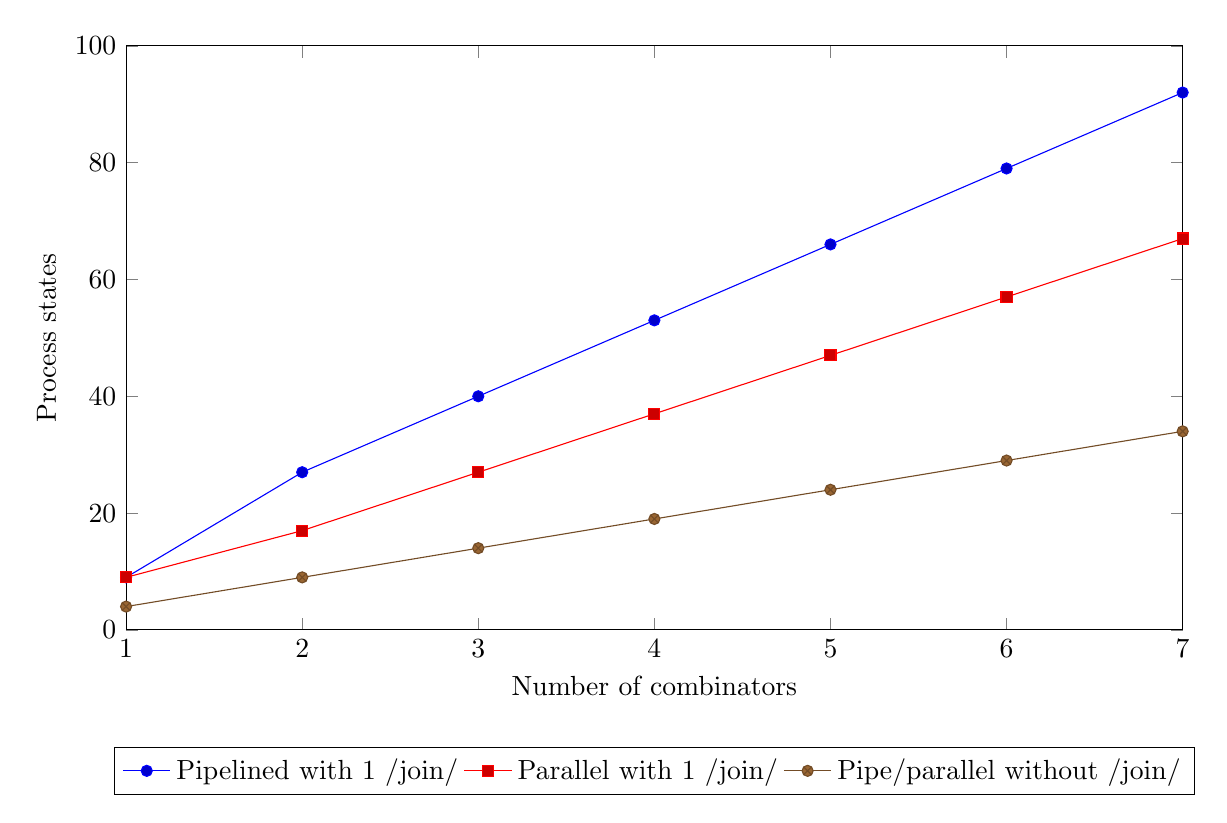
\begin{tikzpicture}
\begin{axis}[
% Hide the label on the second graph
	ylabel=Process states,
	xlabel=Number of combinators,
  ymin=0, ymax=100,
  xmin=1, xmax=7,
  xtick=data,
    width=15cm, height=9.0cm,
    legend style={at={(0.5,-0.2)},anchor=north, legend columns=4},
]
\addplot coordinates {(1,9) (2,27) (3,40) (4,53) (5,66) (6,79) (7,92) };
\addplot coordinates {(1,9) (2,17) (3,27) (4,37) (5,47) (6,57) (7,67) };
\addplot coordinates {(1,4) (2,9) (3,14) (4,19) (5,24) (6,29) (7,34)  };

\legend{Pipelined with 1 \Hs/join/, Parallel with 1 \Hs/join/, Pipe/parallel without \Hs/join/};
\end{axis}
\end{tikzpicture}

\caption{Maximum output process size for fusing all combinations of up to $n$ combinators}
\label{fig:bench:outputsize}
\end{figure}


% -----------------------------------------------------------------------------
\begin{figure}

\begin{tikzpicture}
\begin{axis}[
	ylabel=Process states,
	xlabel=Number of \Hs/join/ combinators,
%  ymode=log,
  ymin=0, ymax=1500,
	enlargelimits=0.01,
  xtick=data,
  xmin=1, xmax=7,
    width=15cm, height=9.0cm,
	legend pos=north west,
]
% These are the values for splitting.
% They are smaller than the 'chaining', but look much nicer on the linear graph.
\addplot coordinates {(1,9) (2,42) (3,97) (4,196) (5,383) (6,746) (7,1461) (8,2880) };

% These are the values for chaining
% \addplot coordinates {(1,4) (2,48) (3,194) (4,760) (5,2814) (6,10064) (7,1) };

\end{axis}
\end{tikzpicture}

\caption{Exponential blowup occurs when splitting or chaining \Hs/join/ combinators together}
\label{fig:bench:exponential}
\end{figure}


